
\section{Results from the GAModel Experiment}

The results of the experiments are in the Table~\ref{gaxriTable} and in the box-plots Figure~\ref{boxPlot2007} and Figure~\ref{boxPlot2009}. The column labelled Random shows the result of the RandomModel, and the idea is the same for the ones labelled GAModel and RI. The ``p-value'' shows the significance value of the {\it Student's t-test} for the null hypothesis `` The mean of the log-likelihood values is greater that the values for RI''.\\

As expected, the RandomModel has lower values than the GAModel. When compared with the RI, the results show that the GAModel is competitive with the RI and that it is promising to use GA to generate earthquake forecasts.\\

\begin{table*}[!ht]
	\begin{center}
		\begin{tabular}{|l|l|c|cc|c|}
			\hline
			\multicolumn{1}{|c|}{Scenario} & \multicolumn{5}{|c|}{Log Likelihood} \\
			\hline
			\multicolumn{1}{|c|}{Year} & \multicolumn{1}{|c|}{Random} & \multicolumn{1}{|c|}{RI} & \multicolumn{2}{c}{GAModel} & \multicolumn{1}{|c|}{p-value} \\    
			\hline
			2000 &-2413.89 &-2124.44 &\raggedright  -2094.05 &\raggedleft (8.80) & 0.01\\%better
			2001 &-2418.14 &-2103.19 &\raggedright  -2101.65 &\raggedleft  (69.49) & 0.57\\%equal
			2002 &-2385.04 &-2094.43 &\raggedright  -2100.01 &\raggedleft (72.62) & 0.07\\%equal
			2003 &-2401.00 &-2104.65 &\raggedright  -2100.76 &\raggedleft (156) & 0.35\\%equal
			2004 &-2421.92 &-2101.92 &\raggedright  -2098.30 &\raggedleft (55.28) & 0.16\\%equal
			2005 &-2643.38 &-2248.40 &\raggedright  -2114.00 &\raggedleft (779) & 0.01\\%better
			2006 &-2616.50 &-2226.93 &\raggedright  -2115.6 &\raggedleft (633) & 0.01\\%better
			2007 &-2451.68 &-2109.13 &\raggedright  -2122.03 &\raggedleft (615) &  0.13\\%equal
			2008 &-2433.23 &-2112.92 &\raggedright  -4435.34 &\raggedleft (657) & 0.14\\%equal
			2009 &-2884.74 &-2438.10 &\raggedright  -2113.1 &\raggedleft (814) & 0.01\\%better
			2010 &-2418.18 &-2114.60 &\raggedright -2112.07 &\raggedleft (843) & 0.79\\%equal
			\hline
		\end{tabular}
	\end{center}
	\caption{Experiments result.}
	\label{gaxriTable}
\end{table*}

\begin{figure}[H]
	\centering
	\begin{minipage}{0.45\textwidth}
		\centering
		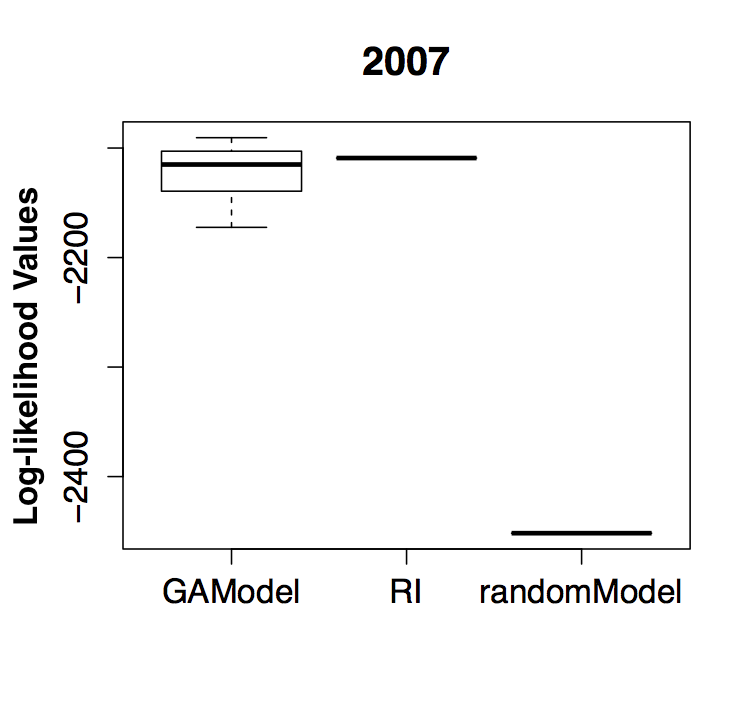
\includegraphics[scale=0.55]{boxPlot2007.png}
		\caption{Box-plot of the values obtained by the models for the year 2007.}
		\label{boxPlot2007}
	\end{minipage}\hfill
	\begin{minipage}{0.45\textwidth}
		\centering
		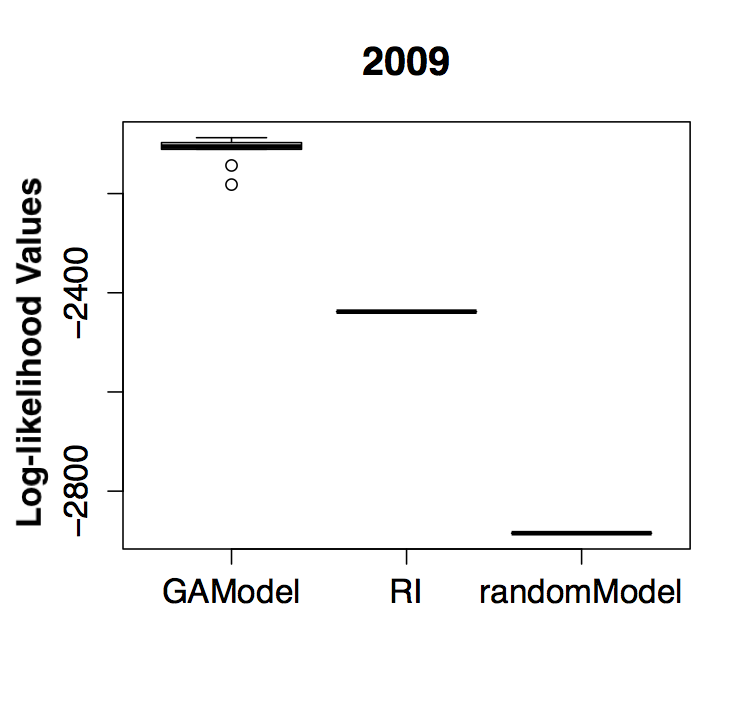
\includegraphics[scale=0.55]{boxPlot2009.png}
		\caption{Box-plot of the values obtained by the models for the year 2009.}
		\label{boxPlot2009}
	\end{minipage}
\end{figure}

\subsection{Models Example and The Real Data}

The Figure~\ref{modeloGAModel} shows a model from the GAModel method for the year 2010. It indicates a low earthquake intensity as green while the more intensity areas, are shown as orange (for even higher cases, white is used). The Figure~\ref{modeloRI} shows a model from the RI Algorithm for the year 2010. It indicates a low earthquake intensity as white while the more intensity areas, are shown in red. For comparison reasons, we show the Figure~\ref{realData}, that shows the earthquake occurrences for the same year.\\


\begin{figure}[H]
	\centering
	\begin{minipage}{0.45\textwidth}
		\centering
		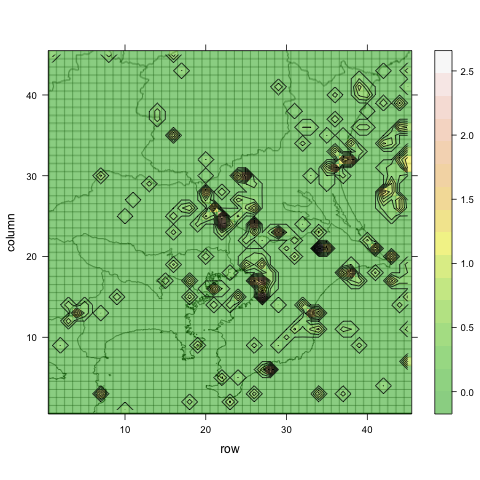
\includegraphics[scale=0.4]{media2010.png}
		\caption{ GAModel model for the year of 2010 in Kanto.}
		\label{modeloGAModel}
	\end{minipage}\hfill
	\begin{minipage}{0.45\textwidth}
		\centering
			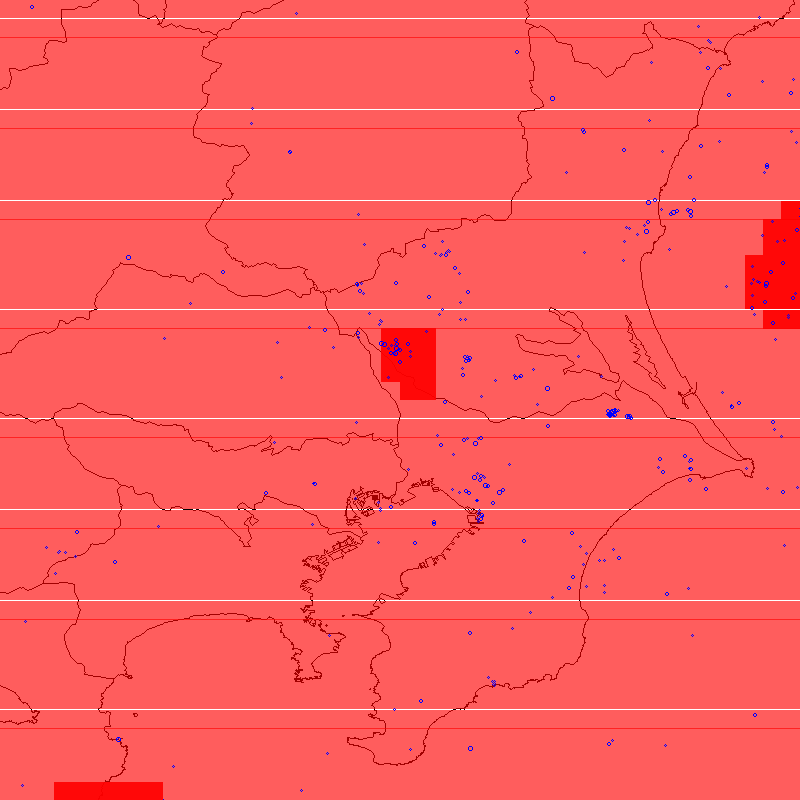
\includegraphics[scale=0.18]{kanto10_RI.png}
			\caption{RI model for the year of 2010 in Kanto. Figure from~\cite{ecta14}.}
			\label{modeloRI}
	\end{minipage}
\end{figure}

\begin{figure}[H]
		\centering
		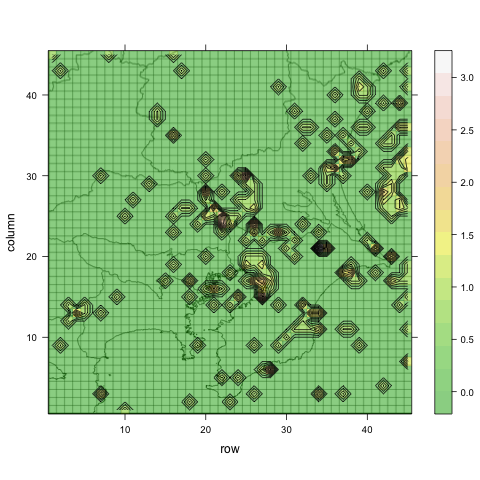
\includegraphics[scale=0.4]{matriz2010_real.png}
		\caption{Earthquake occurrences in the year of 2010 in Kanto.}
		\label{realData}
\end{figure}


\section{Results from The Main-shock Models Main-shock with After-shock Models Experiment}\label{resultsBigExp}

An one-way between subjects ANOVA was conducted to compare the effects of the models, the depths, the years and regions on the log-likelihood value. In this study there are the models: ReducedGAModel, GAModel, Emp-GAModel, Emp-ReducedGAModel, GAModelWindow, ReducedGAModelWindow, GAModelSLC, ReducedGAModelSLC, Emp-GAModelClustered, Emp-ReducedGAModelWindow, Emp-GAModelSLC and Emp-ReducedGAModelSLC.  \\

Based on the results of this first test, it is evident that all variables are significantly different. The results of the experiments are in the Table~\ref{anovatest1}. For all, the confidence interval is set to 5\%.\\

The column labelled Random shows the result of the RandomModel, and the idea the is same for the ones labelled GAModel and RI. The ``p-value'' shows significance value of the {\it Student's t-test} for null hypothesis `` The mean of the log-likelihood values is greater that the values for RI''.\\

\begin{table*}[!ht]
	\centering
	\begin{tabular}{|l|l|l|l|l|l|}
		\hline
		{Variable} & {Degrees of Freedom} & {Sum Sq}    & {Mean Sq}   & {F Value} & {Pr(\textgreater F)} \\
		\hline
		Model    & 11           	  & 1.984e+08  & 18035604   & 113.87    & \textless2e-16     \\
		\hline
		Depth    & 2                  & 2.955e+07  & 14772789   & 93.27     & \textless2e-16     \\
		\hline
		Year     & 5                  & 1.065e+09  & 213025401  & 1344.95   & \textless2e-16     \\
		\hline
		Region   & 3                  & 2.188e+09  & 729443498  & 4605.38   & \textless2e-16	\\    
		\hline
	\end{tabular}
	\caption{Simple ANOVA Test Results.}
	\label{anovatest1}
\end{table*}


Because we found statistically significant result, we applied a Post hoc comparisons using the Tukey HSD test. It compared each condition with all others. For example, it compares the values from the GAModel with the GAModelWindow, see Figure~\ref{modelANOVA}. It indicated that the models that used the catalogues from the Window Method or the Single Link Cluster, when compared with all other models, achieve greater log-likelihood values. Furthermore, we noticed that the depths conditions show a greater influence when the depth in smaller or equal to 25 km, see Figure~\ref{depthsANOVA}.\\

\begin{figure}[H]
	\centering
	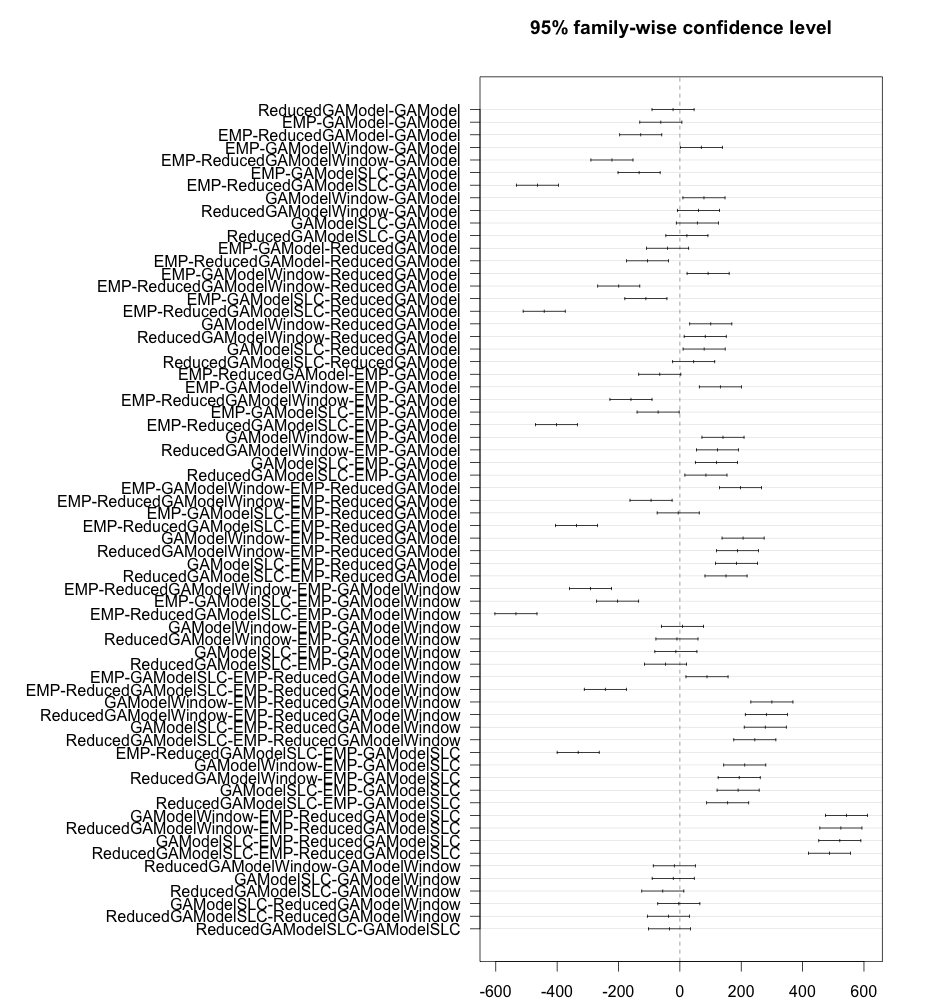
\includegraphics[scale=0.45]{1modelANOVA.png}
	\caption{ANOVA results - Models.}
	\label{modelANOVA}
\end{figure}

\begin{figure}[H]
	\centering
	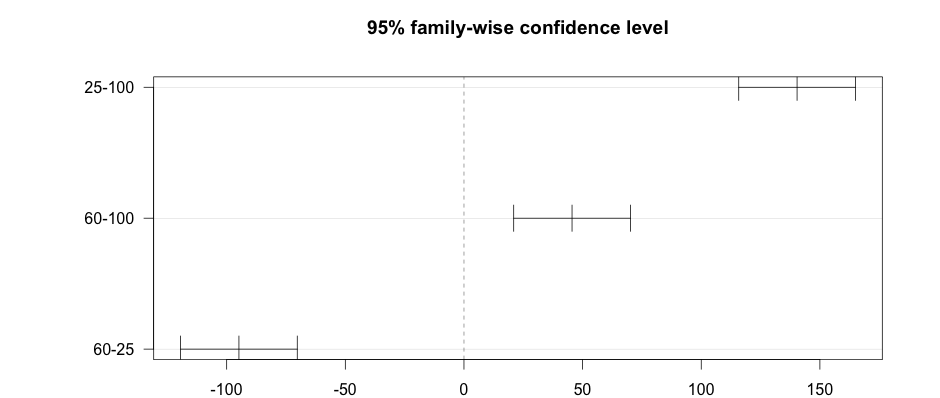
\includegraphics[scale=0.45]{depthsClusterANOVA.png}
	\caption{ANOVA results - Depths.}
	\label{depthsANOVA}
\end{figure}

Then, we decided to compare only the those models against themselves. That is, models used for this new comparison are those that used the catalogues from the Window Method or the Single Link Cluster and with earthquakes with depth smaller or equal to 25 km.\\

\begin{table*}[!ht]
	\centering
	\begin{tabular}{|l|l|l|l|l|l|}
		\hline
		{Variable} & {Degrees of Freedom} & {Sum Sq}    & {Mean Sq}   & {F Value} & {Pr(\textgreater F)} \\
		\hline
		Model    & 7            	  & 21991488   & 3141641    & 21.07     & \textless2e-16     \\
		\hline
		Year     & 5                  & 240753808  & 48150762   & 322.94    & \textless2e-16     \\
		\hline
		Region   & 3                  & 374602684  & 124867561  & 837.48    & \textless2e-16	\\    
		\hline
	\end{tabular}
	\caption{Simple ANOVA Test Results.}
	\label{anovatest2}
\end{table*}

Based on the results of this test, it is evident that all variables are still significantly different. The results of the experiments are in the Table~\ref{anovatest2}. For all, as before, the confidence interval is set to 5\%.\\


Again, we found statistically significant result, therefore, we applied the Tukey HSD test. The results are shown in Figure~\ref{modelANOVA2}. It indicated that the models from the GAModel method, when compared with all other models, achieve greater log-likelihood values.\\

\begin{figure}[H]
	\centering
	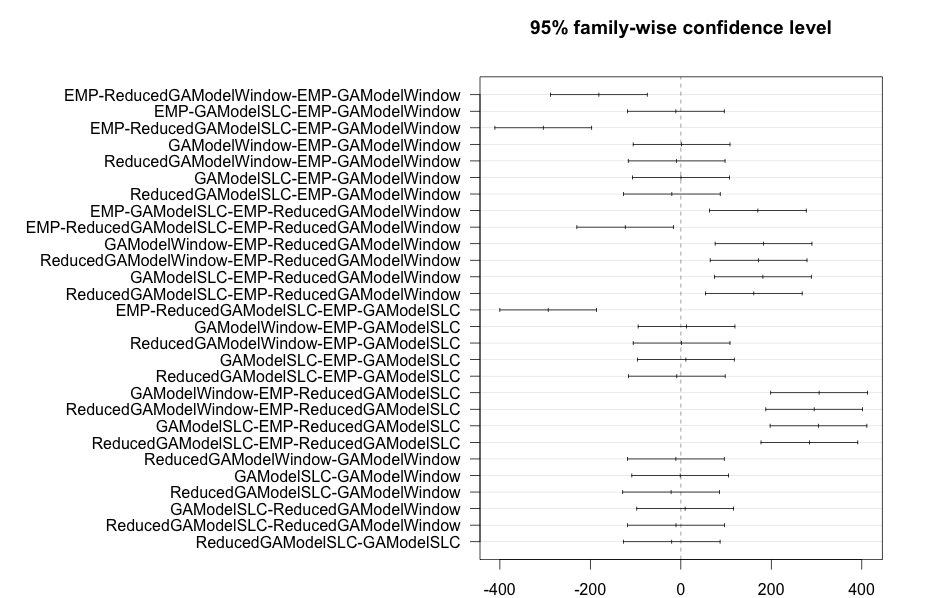
\includegraphics[scale=0.45]{2modelANOVA.png}
	\caption{ANOVA results - Models.}
	\label{modelANOVA2}
\end{figure}

Based on the last results, we performed the ANOVA again, comparing only models from the GAModel method. The results of the experiments are in the Table~\ref{anovatest3}.\\

\begin{table*}[!ht]
	\centering
	\begin{tabular}{|l|l|l|l|l|l|}
		\hline
		{Variable} & {Degrees of Freedom} & {Sum Sq}    & {Mean Sq}   & {F Value} & {Pr(\textgreater F)} \\
		\hline
		Model    & 3            	  & 24462      & 8154       & 0.058      &  0.981      \\
		\hline
		Year     & 5                  & 121287074  & 24257415   & 173.600    & \textless2e-16     \\
		\hline
		Region   & 3                  & 167719464  & 55906488   & 400.099    & \textless2e-16	\\    
		\hline
	\end{tabular}
	\caption{Simple ANOVA Test Results.}
	\label{anovatest3}
\end{table*}

This time, we found statistically significant result only for the year and region condition. To show that the models results are not statistically different from each other, we applied a pairing analysis.\\

From the the pairing analysis, we decided to use the \textit{GAModelWindow} as the representative method of this study. That is because, in most cases when its values were compared, it showed a little better performance in the means of the log-likelihood values. For the results, see the Table~\ref{Paired}.\\

\begin{table*}[!ht]
	\begin{center}
		\begin{tabular}{|l|l|c|cc|c|}
			\hline
			\multicolumn{1}{|c|}{Scenario} & \multicolumn{5}{|c|}{Log Likelihood} \\
			\hline
			\multicolumn{1}{|c|}{Models} & \multicolumn{1}{|c|}{Kansai} & \multicolumn{1}{|c|}{Touhoku} & \multicolumn{2}{c}{East Japan} & \multicolumn{1}{|c|}{Kanto} \\    
			\hline
			EMP-GAModelWindow &-2643.38 &-2248.40 &\raggedright  -2114.00 &\raggedleft (779) & 0.01\\%better
			2006 &-2616.50 &-2226.93 &\raggedright  -2115.6 &\raggedleft (633) & 0.01\\%better
			2007 &-2451.68 &-2109.13 &\raggedright  -2122.03 &\raggedleft (615) &  0.13\\%equal
			2008 &-2433.23 &-2112.92 &\raggedright  -4435.34 &\raggedleft (657) & 0.14\\%equal
			2009 &-2884.74 &-2438.10 &\raggedright  -2113.1 &\raggedleft (814) & 0.01\\%better
			2010 &-2418.18 &-2114.60 &\raggedright -2112.07 &\raggedleft (843) & 0.79\\%equal
			\hline
		\end{tabular}
	\end{center}
	\caption{Experiments result.}
	\label{Paired}
\end{table*}


%TODO: add ALL figures
\subsection{The Models Examples And The Real Data}

The Figure~\ref{gamodel2005eastjapan} shows a model from the GAModel method for the year 2005 in East Japan. The next Figure,~\ref{reduced2005eastjapan} shows a model from the ReducedGAModel~\ref{reducedGAModel} method for the year 2005 in East Japan.\\

All Figures,~\ref{gamodel2005eastjapan}~\ref{reduced2005eastjapan}~\ref{hybridgamodel2005eastjapan}~\ref{hybridreduced2005eastjapan},  indicate a low earthquake intensity as white while the more intensity areas, are shown in red. They are, in order, the data visualisation for the model from: the GAModel, the ReducedGAModel, the Emp-GAModel and the Emp-ReducedGAModel for East Japan in 2005. The Figure~\ref{real2005eastjapan} represents the earthquake occurrences in the same region and year.\\


\begin{figure}[H]
		\centering
		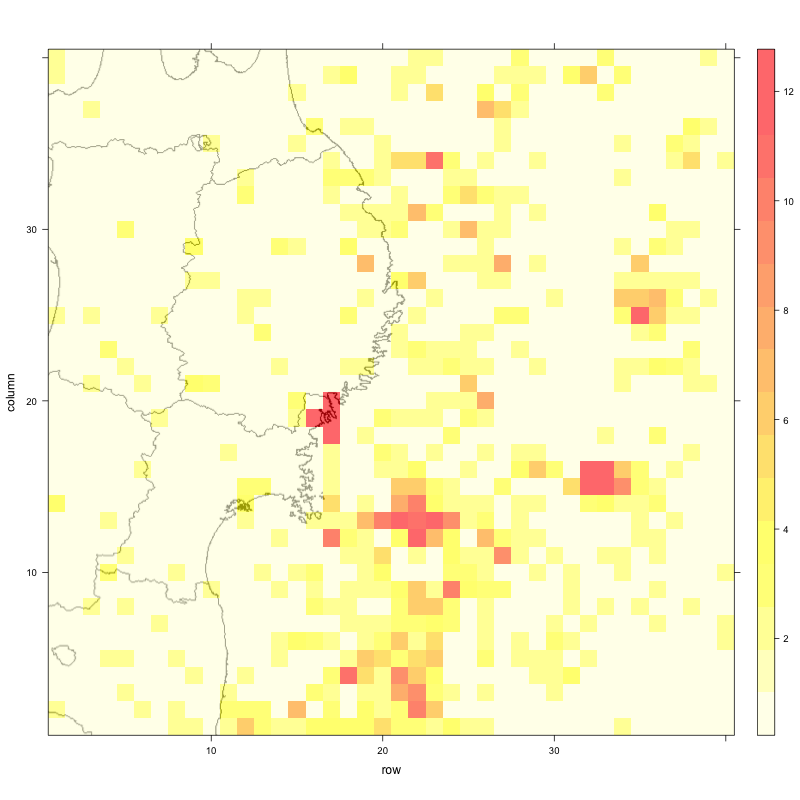
\includegraphics[scale=0.2]{real2005eastjapan.png}
		\caption{Earthquake occurrences in the year of 2005 in East Japan.}
		\label{real2005eastjapan}
\end{figure}


\begin{figure}[H]
	\centering
	\begin{minipage}{0.45\textwidth}
		\centering
		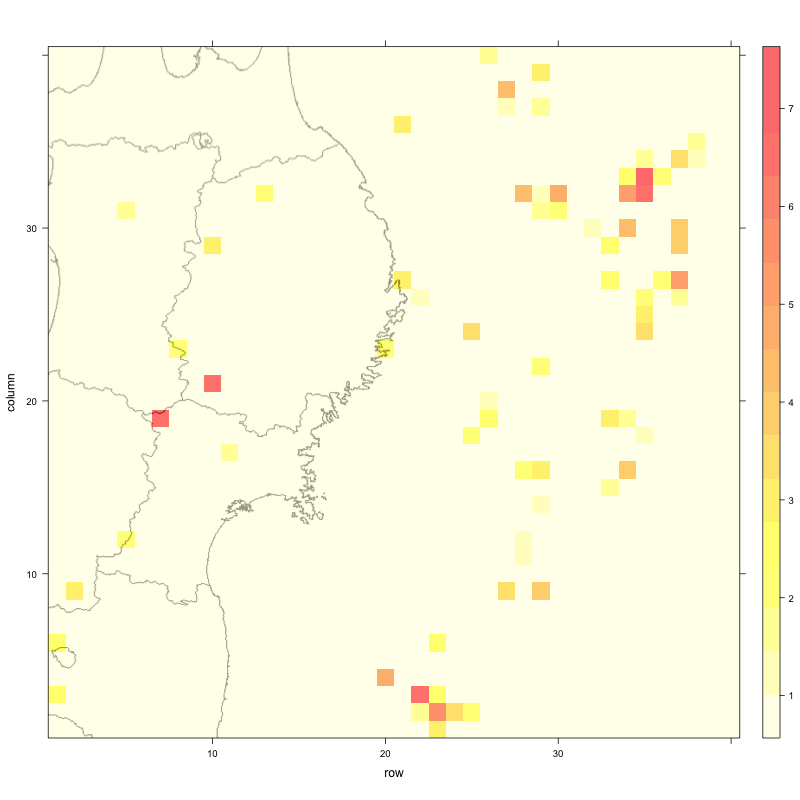
\includegraphics[scale=0.2]{reduced2005eastjapan.png}
		\caption{ReducedGAModel model - year of 2005, East Japan.}
		\label{reduced2005eastjapan}
	\end{minipage}
	\begin{minipage}{0.45\textwidth}
		\centering
		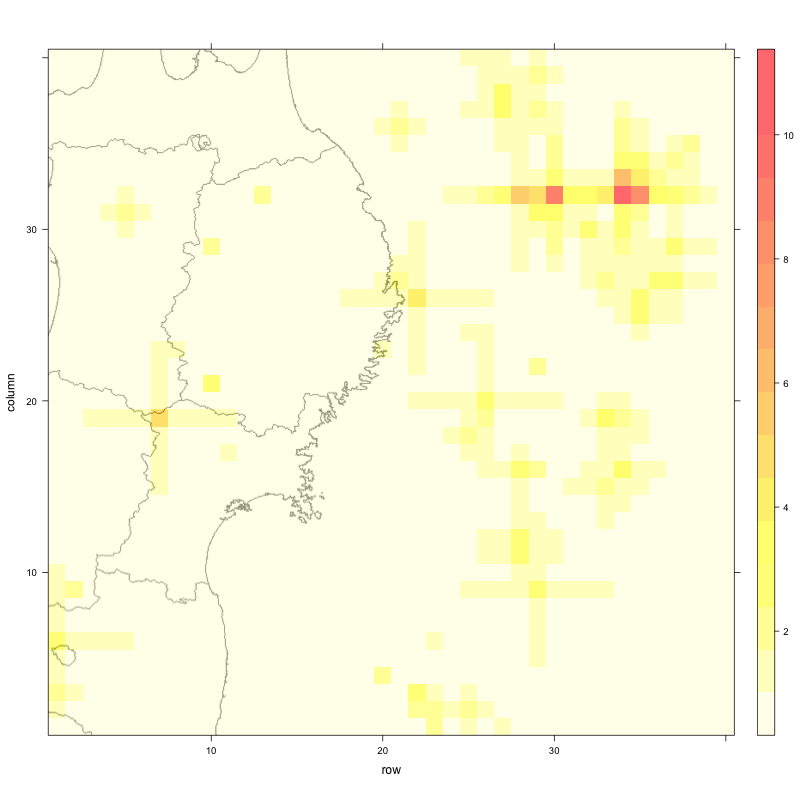
\includegraphics[scale=0.2]{hybridgamodel2005eastjapan.png}
		\caption{Em-GAModel model - year of 2005, East Japan.}
		\label{hybridgamodel2005eastjapan}
	\end{minipage}
\end{figure}

\begin{figure}[H]
	\begin{minipage}{0.45\textwidth}
		\centering
			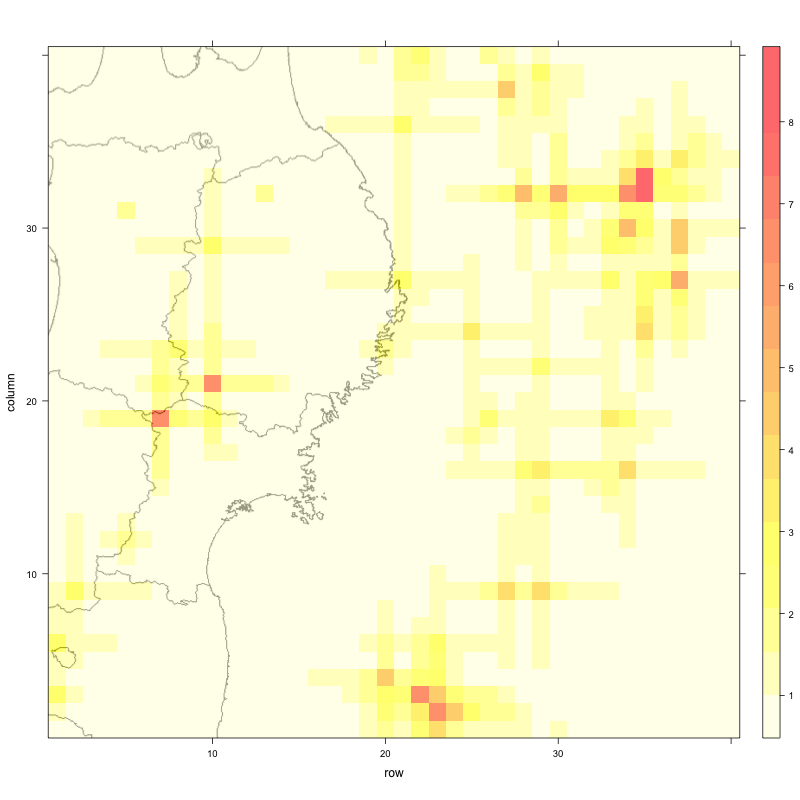
\includegraphics[scale=0.2]{hybridreduced2005eastjapan.png}
			\caption{Emp-ReducedGAModel model - year of 2005, East Japan.}
			\label{hybridreduced2005eastjapan}
	\end{minipage}
	\begin{minipage}{0.45\textwidth}
		\centering
		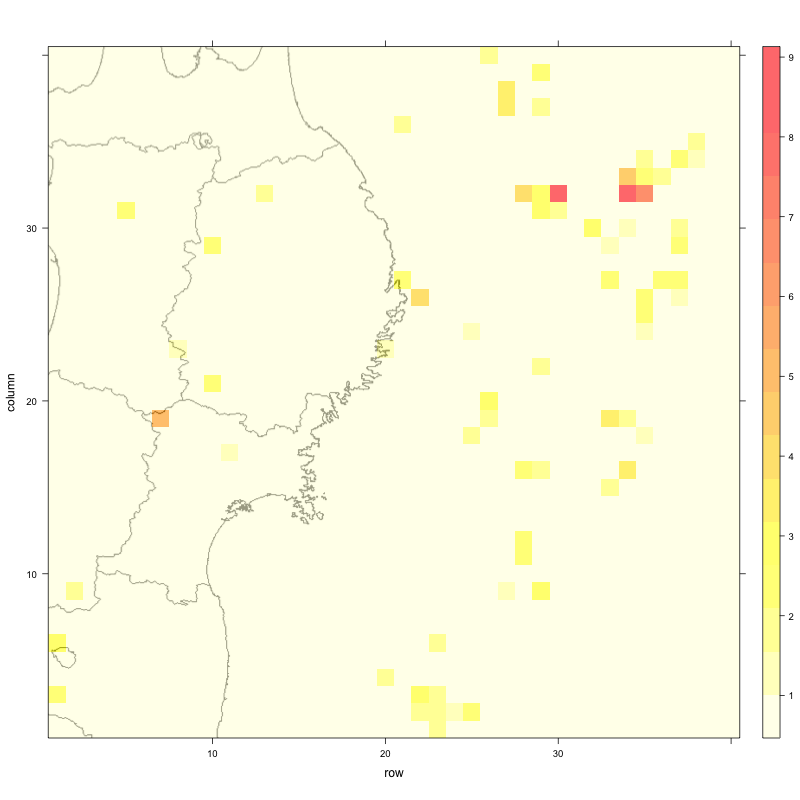
\includegraphics[scale=0.2]{gamodel2005eastjapan.png}
		\caption{GAModel model - year of 2005, East Japan.}
		\label{gamodel2005eastjapan}
	\end{minipage}
\end{figure}

%TODO: add magnitude study!
\section{Magnitude Study}
From the results already obtain and showed in the section~\ref{resultsBigExp}, when selected the models with earthquakes with depth smaller or equal to 25 km and then we split the models in magnitude intervals, as defined in~\ref{magExp}.\\

After that, we compared those split models against themselves. Based on the results of this test, it is evident that all variables are still significantly different. The results of the experiments are in the Table~\ref{anovatestMag}. For all, as before, the confidence interval is set to 5\%.\\

\begin{table*}[!ht]
	\centering
	\begin{tabular}{|l|l|l|l|l|l|}
		\hline
		{Variable} & {Degrees of Freedom} & {Sum Sq}    & {Mean Sq}   & {F Value} & {Pr(\textgreater F)} \\
		\hline
		Model       & 5            	  & 2.368e+09      & 4.737e+08    & 3058     & \textless2e-16     \\
		\hline
		Year        & 3                  & 4.139e+09   & 1.380e+09    & 8906     & \textless2e-16     \\
		\hline
		Magnitude   & 7                  & 3.212e+09   & 4.588e+08    & 2962     & \textless2e-16	\\    
		\hline
	\end{tabular}
	\caption{Simple ANOVA Test Results.}
	\label{anovatestMag}
\end{table*}

We found statistically significant result and, as before, we applied the Tukey HSD test. The results are shown in Figure~\ref{modelANOVAMag} and the \textit{NULL} field was used as the model with all magnitude intervals (the complete model).\\

It indicated that the interval $[3.0-4.0]$ always performed, in terms of log-likelihood values, worse than all other intervals. this phenomenon also happens in the interval $[4.0-5.0]$, though in this case, the difference is not as big as the last one. The other intervals show no significant difference.\\

From the results found, we decided to chose only earthquakes with magnitude higher than 4.0 as our threshold value.\\

\begin{figure}[H]
	\centering
	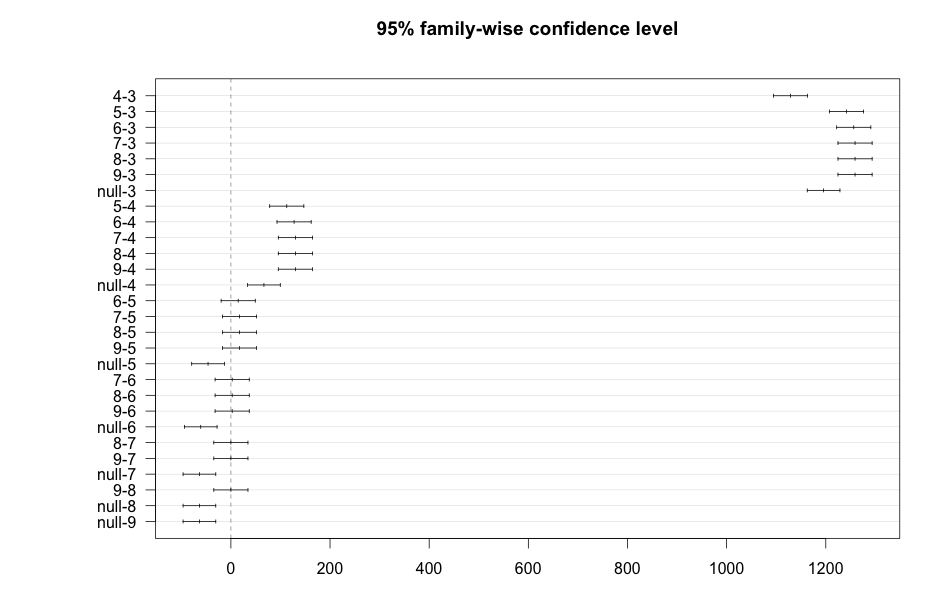
\includegraphics[scale=0.45]{magModels.png}
	\caption{ANOVA results - Models.}
	\label{modelANOVAMag}
\end{figure}



%magModels.png,magyears.png, magRegions.png